\documentclass{article}
\usepackage[utf8]{inputenc}
\usepackage[margin=0.4in]{geometry}


\title{Computer Networks HW 4}
\author{Shane Cincotta }
\date{April 27, 2020}

\usepackage{natbib}
\usepackage{graphicx}

\begin{document}

\maketitle

\section*{Chapter 3, Review Question 14}
\subsection*{a} False.\\
\subsection*{b} False.\\
\subsection*{c} True.\\
\subsection*{d} False.\\
\subsection*{e} True.\\
\subsection*{f} False.\\
\subsection*{g} False.\\

\section*{Chapter 3, Review Question 15}
\subsection*{a} 20 Bytes.\\
\subsection*{b} 90.\\

\section*{Chapter 3, Review Question 18}
False.\\

\section*{Chapter 3, Problem 26}
\subsection*{a} MSS = 4bytes = 32 bits, thus L=$2^{32}$.\\
\subsection*{b} Number of segments = $\frac{2^{32}}{536}$ = 8012998.6865 bytes.\\
\newline Total bytes sent over 155 Mbps link = 8012998.6865 * 66 = 528857913.313 bytes.\\
\newline Total number of bytes to be transmitted = $2^{32} + 528857913.313$ = 4.824 * $10^9$.\\
\newline Thus it would take $\frac{4.36107 * 10 ^9 * 8}{155*10^6}$ seconds.\\
\newline $\frac{4.36107 * 10 ^9 * 8}{155*10^6}$ = 248.98 seconds.\\

\section*{Chapter 3, Problem 27}
\subsection*{a} Sequence number = 127 + 80 = 207, source port = 302, destination port = 80.\\
\subsection*{b} ACK number = 207, source port = 80 and destination port = 302.\\
\subsection*{c} The ACK number will be 127.\\
\subsection*{d}

\begin{figure}[h!]
\centering
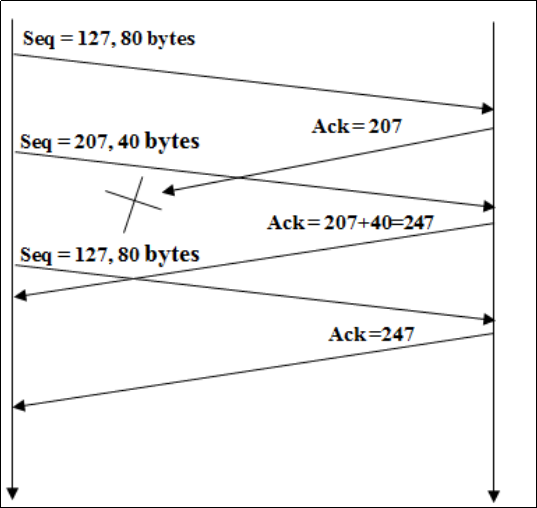
\includegraphics[scale=0.35]{P27.png}
\end{figure}

\clearpage

\section*{Chapter 3, Problem 31}
\subsection*{a}  $EstimatedRTT_{106} = (1-a)*EstimatedRTT + a * SampleRTT$.\\
\newline $= (1-0.125) * 100 + 0.125*106$.\\
\newline $= 100.75$.\\
\newline $DevRTT_{106} = (1-b) * DevRTT + b | SampleRTT -EstimatedRTT|$.\\
\newline $= (1-0.25) * 5 + 0.25 * |106-100.75|$.\\
\newline $= 5.06$.\\
\newline $TimeoutInterval_{106} = EstimatedRTT + 4 * DevRTT$.\\
\newline $= 120.99$.\\

\subsection*{b}  $EstimatedRTT_{120} = (1-a)*EstimatedRTT + a * SampleRTT$.\\
\newline $= (1-0.125) * 100.75 + 0.125*120$.\\
\newline $= 103.15$.\\
\newline $DevRTT_{120} = (1-b) * DevRTT + b | SampleRTT -EstimatedRTT|$.\\
\newline $= (1-0.25) * 5.06 + 0.25 * |120-103.15|$.\\
\newline $= 8$.\\
\newline $TimeoutInterval_{120} = EstimatedRTT + 4 * DevRTT$.\\
\newline $= 135.15$.\\

\subsection*{c}  $EstimatedRTT_{140} = (1-a)*EstimatedRTT + a * SampleRTT$.\\
\newline $= (1-0.125) * 103.15 + 0.125*140$.\\
\newline $= 107.756$.\\
\newline $DevRTT_{140} = (1-b) * DevRTT + b | SampleRTT -EstimatedRTT|$.\\
\newline $= (1-0.25) * 8 + 0.25 * |140-107.756|$.\\
\newline $= 14.061$.\\
\newline $TimeoutInterval_{140} = EstimatedRTT + 4 * DevRTT$.\\
\newline $= 164$.\\

\subsection*{d}  $EstimatedRTT_{90} = (1-a)*EstimatedRTT + a * SampleRTT$.\\
\newline $= (1-0.125) * 107.756 + 0.125*90$.\\
\newline $= 105.536$.\\
\newline $DevRTT_{90} = (1-b) * DevRTT + b | SampleRTT -EstimatedRTT|$.\\
\newline $= (1-0.25) * 14.061 + 0.25 * |90-105.54|$.\\
\newline $= 14.43$.\\
\newline $TimeoutInterval_{90} = EstimatedRTT + 4 * DevRTT$.\\
\newline $= 163.256$.\\

\subsection*{e}  $EstimatedRTT_{115} = (1-a)*EstimatedRTT + a * SampleRTT$.\\
\newline $= (1-0.125) * 105.536 + 0.125*115$.\\
\newline $= 106.72$.\\
\newline $DevRTT_{115} = (1-b) * DevRTT + b | SampleRTT -EstimatedRTT|$.\\
\newline $= (1-0.25) * 14.43 + 0.25 * |115-106.72|$.\\
\newline $= 12.89$.\\
\newline $TimeoutInterval_{115} = EstimatedRTT + 4 * DevRTT$.\\
\newline $= 158.28$.\\

\section*{Chapter 3, Problem 33}
The sample RTT ACK from packet A may be congested in the network possibly due to queueing delays.  It is also possible to know the number of segments that are transmitted but it is not possible to know the number of segments that are retransmitted.  So while calculating EstimatedRTT. SampleRTT doesn't need to be considered. Since SampleRTT for unknown number of retransmitted segments cannot be traced, EstimatedRTT for retransmitted segments is not considered.\\

\section*{Chapter 3, Problem 36}
At the reciever, when out-of-order segments with higher-than-expected sequence number arrives, a gap is detected.  The reciever then sends a duplicate ACK for the already received segment.  A sender often sends a large number of segments back to back.  If one segment is lost, there will be many back-to-back duplicate ACKs.\\

\section*{Chapter 3, Problem 44}
\subsection*{a}
The TCP's transmission rate is $\frac{w}{RTT}$.\\
\newline It takes 6 RTTs to increase cwnd 12 MSS.\\

\subsection*{b}
By 6 RTTs, 51 MSS were sent and acknowledged.  Thus the average throughput up to time 6 RTT is $\frac{51}{6}$ = 8.5 MSS/RTT.

\end{document}